\chapter{The CMS experiment at the \LHC}
\label{chap:detector}

% \chapterquote{There, sir! that is the perfection of vessels!}
% {Jules Verne, 1828--1905}

To be able to reliably probe the energy scales at which the \SM breaks
down, one of the largest machines ever built was constructed in a
27~km ring underground on the border of France and Switzerland: the
\LHC. Along this are built a series of detectors that can record in a high
level of detail the result of high energy particle collisions produced
by this collider. This chapter will focus on the details and
performance of \CMS, a multi-purpose detector optimised to search for
new, as yet undiscovered, particles.

\section{The \LHC}
\label{sec:lhc}

The \LHC is a hadron collider designed to collide protons and lead
ions at centre of mass energies up to 14\tev, the highest ever achieved by such a
machine
\cite{Evans:2008zzb,CERN-2004-003-V-1,CERN-2004-003-V-2,CERN-2004-003-V-3}.
The proton-proton collisions are most utilised for direct searches for
new physics and therefore take up the vast majority of the \LHC's
running time. 

To bring protons up to the $6.5\tev$ required in Run~2 of the \LHC they are
accelerated through a series of stages. Hydrogen atoms are initially stripped
of their electrons and accelerated to 50\mev by a linear accelerator,
\ac{LINAC2}. The energy is then increased to 1.4\gev by the \ac{PSB} before
being injected into the \ac{PS} which brings the energies up to 26\gev. A final
kick up to 450\gev is provided by the \ac{SPS}. This chain of accelerators also
collect the protons into bunches that are either 25~ns (from Run~2 onwards) or
50~ns apart (during Run~1 and early stages of Run~2). These bunches are then
injected into the \LHC, in which they are steered by around 1200
superconducting dipole magnets while being accelerated up to $6.5\tev$ with
\ac{RF} cavities. Once the beam has reached the intended energy and is stable,
protons are collided at four different points on the ring, around which are
built the four major \LHC detectors, ALICE \cite{Aamodt:2008zz}, ATLAS
\cite{Aad:2008zzm}, LHCb \cite{Alves:2008zz} and \CMS \cite{Chatrchyan:2008aa}.
A representation of this accelerator complex and the location of the
detectors can be seen in Fig.~\ref{fig:lhc}.

\begin{figure}
  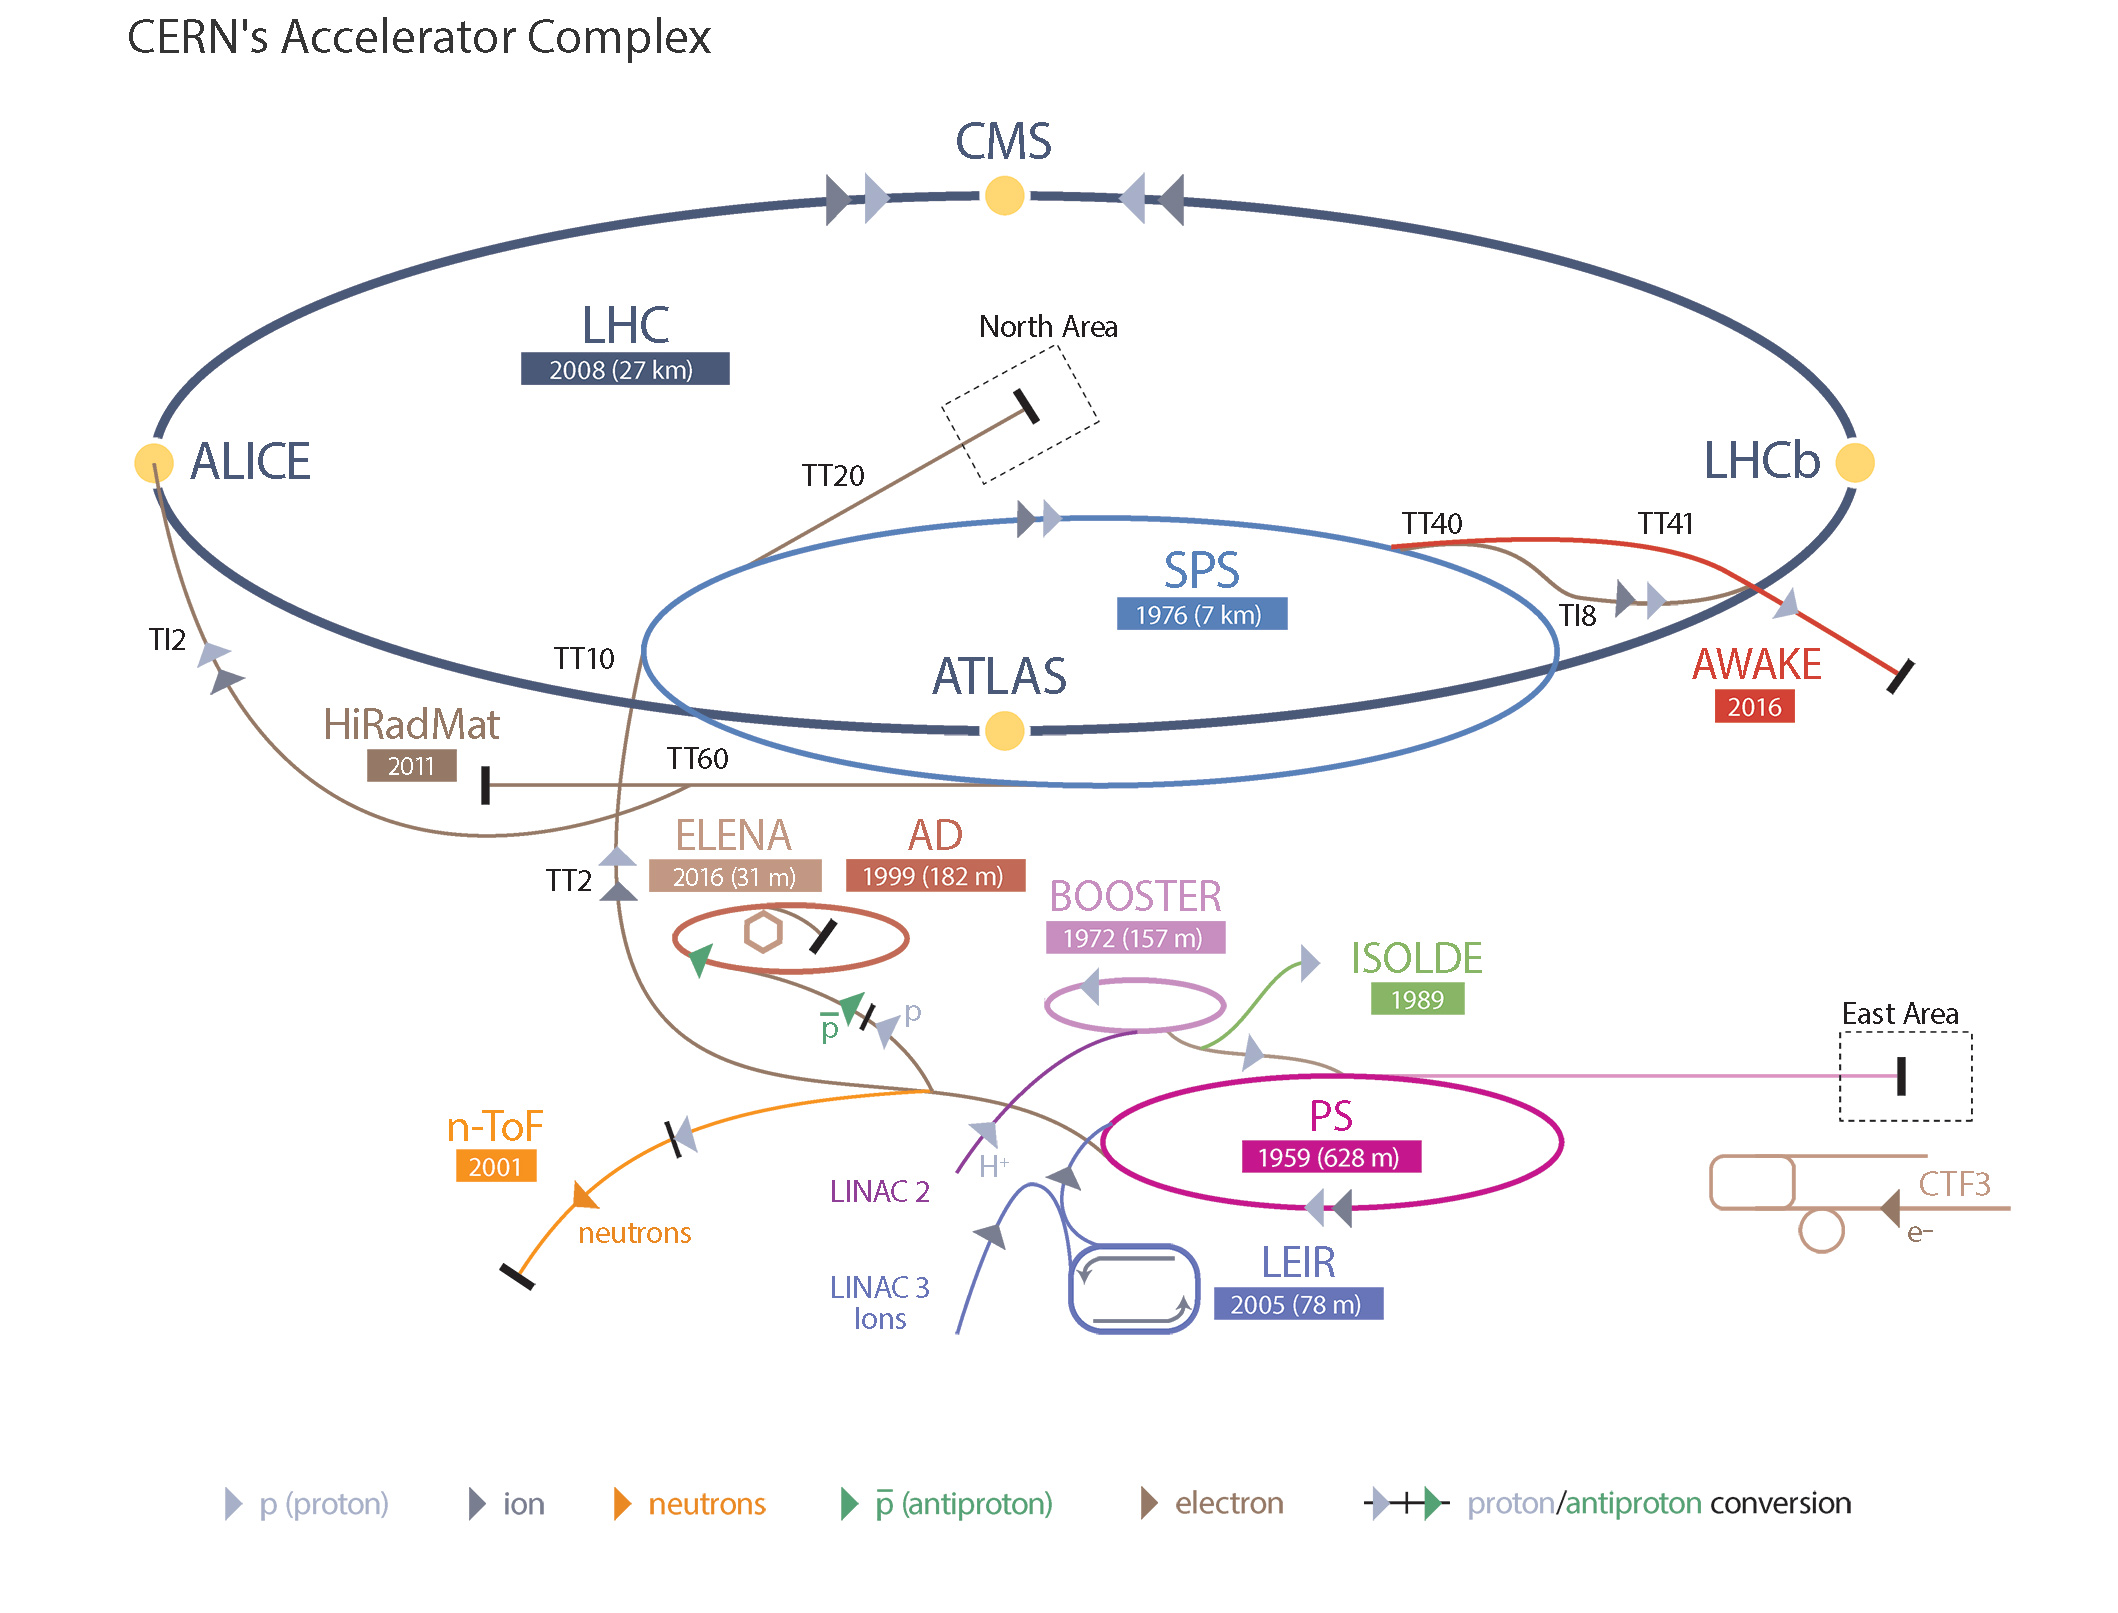
\includegraphics[width=\largefigwidth]{figs/LHC_default}
  \caption[]%
  {A representation of the CERN accelerator complex that help
  accelerate protons to record energies within the \LHC
  \cite{stfc:lhc}}%
  \label{fig:lhc}
\end{figure}

As well as attaining record breaking energies, the \LHC is designed to
collide hadrons at a very high luminosity, with a bunch collision rate
up to $40\mhz$ \cite{Evans:2008zzb}. The necessity of this is demonstrated in
Fig.~\ref{fig:xsecs}. The rate at which electroweak scale processes
occur in proton collisions is significantly lower than their
associated backgrounds. The \LHC is therefore designed to run at a
maximum instantaneous luminosity of $10^{34}$cm$^{-2}$s$^{-1}$ to
maximise the occurence of rare high energy processes. Along with
the high collision rate, this luminosity is achieved by squeezing the
proton bunches to increase the number of simultaneous collisions per
bunch crossing, the extra simultaneous collisions are known as \PU.

\begin{figure}
  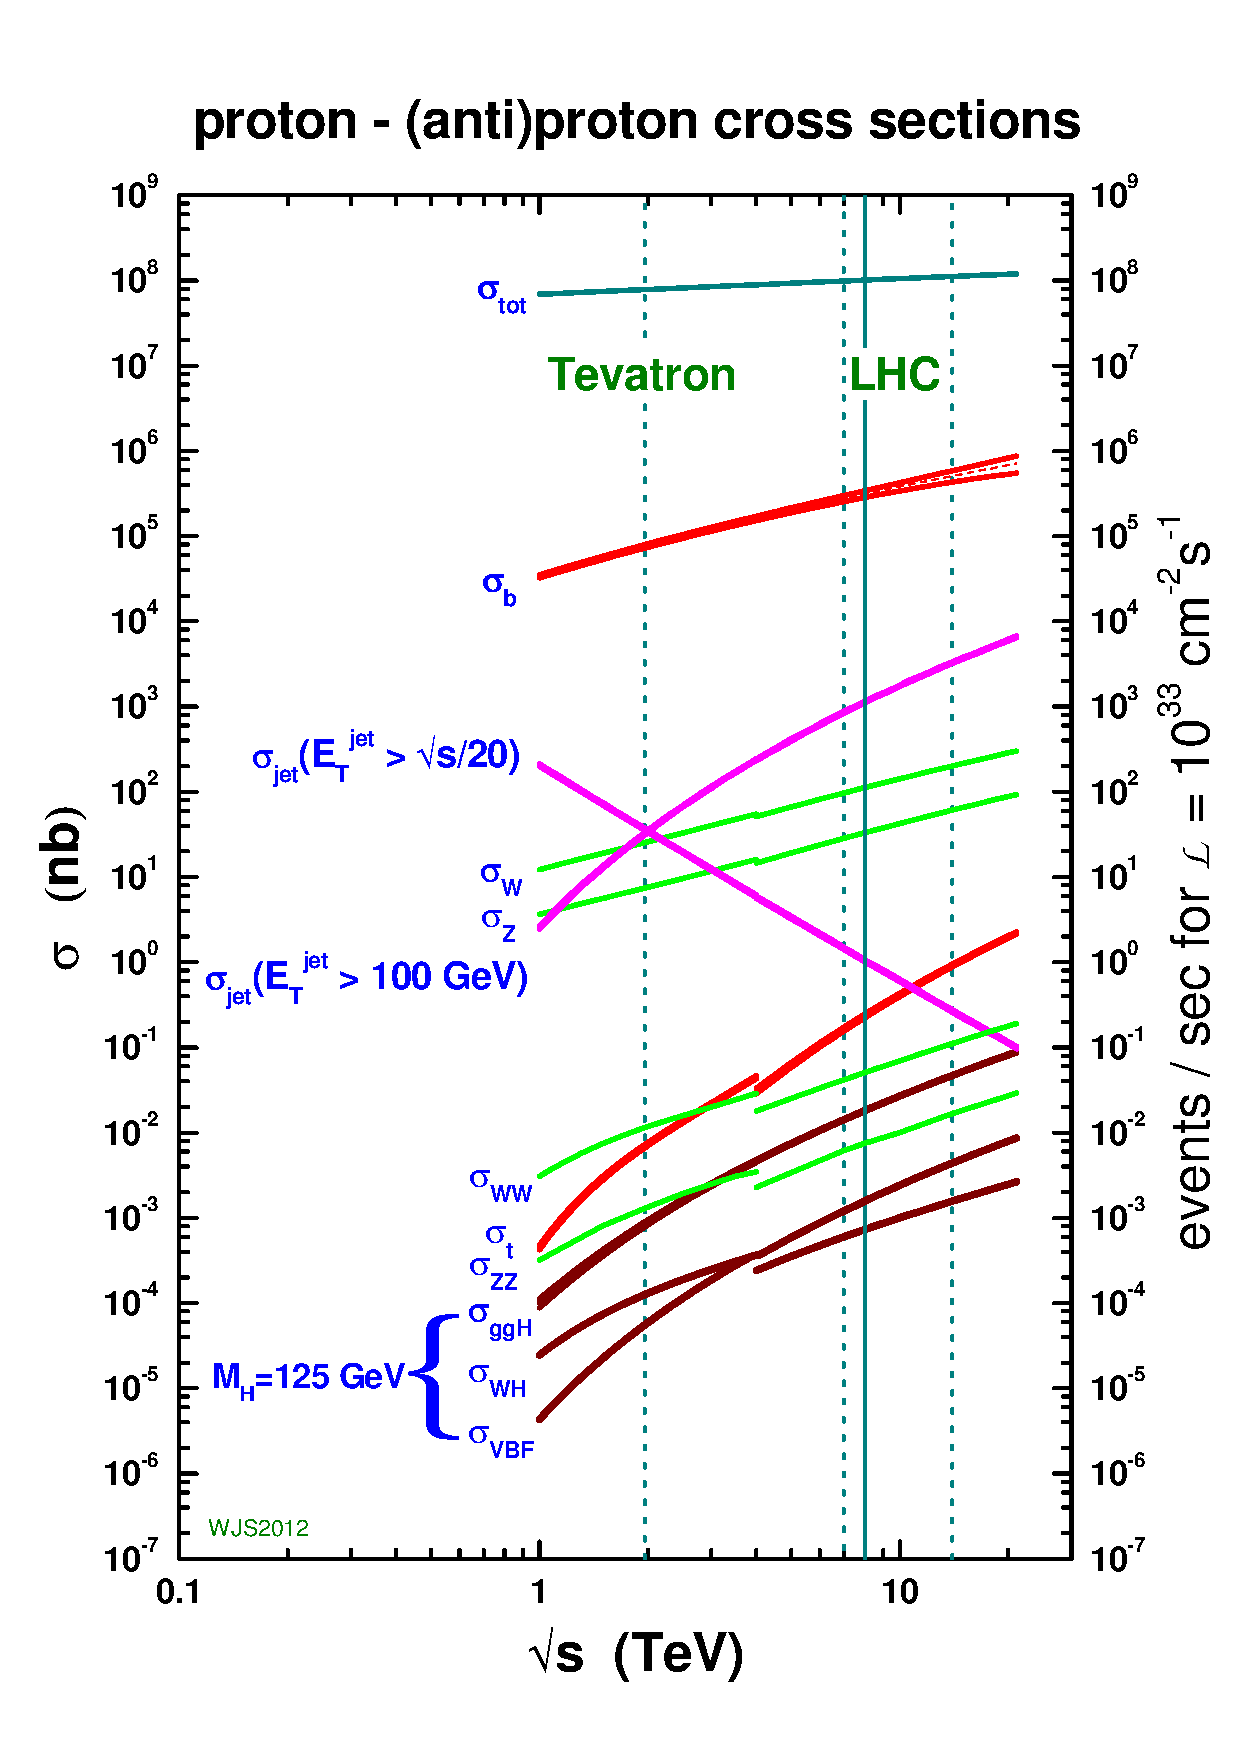
\includegraphics[width=\mediumfigwidth]{figs/crosssections2012_v5}
  \caption[]%
  { The cross sections for various standard model processes as a
  function of proton collider energy, demonstrating the importance of
  high luminosities when observing electroweak scale processes
  \cite{stirlingCrossSec1}.}%
  \label{fig:xsecs}
\end{figure}

During Run~1 of the \LHC, from 2010-2013, a total of $23.3\ifb$ of
data were collected at energies of $\sqrt{s}=7\tev$ and $8\tev$. After
this there was a period of shutdown in which the \LHC and the
detectors underwent a series of upgrades. Run~2 then began in 2015
with the collision of protons at $\sqrt{s}=13\tev$. During 2015 a
total of $4.3\ifb$ were collected at this energy. So far in 2016 the
\LHC has delivered $34.6\ifb$, a record breaking number of collisions
at the highest ever recorded energies.

% \begin{figure}
%   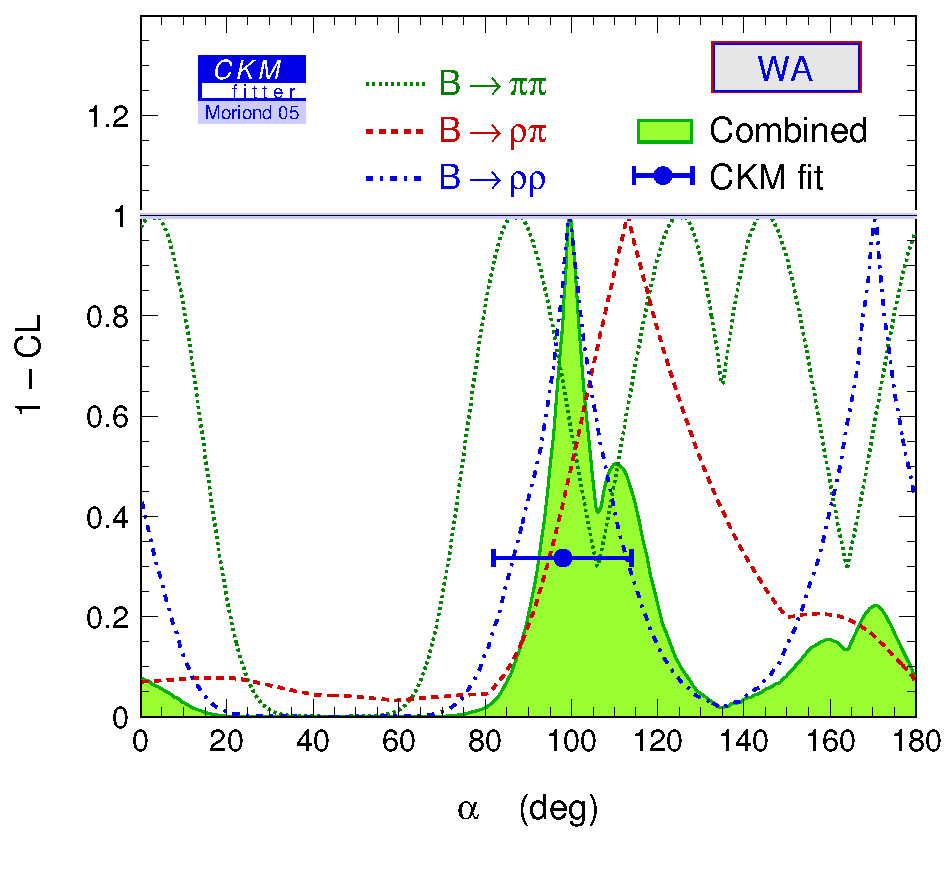
\includegraphics[width=\largefigwidth]{ckmfitter-alpha-combined}
%   \caption[CKM Fitter constraints on \alphaCKM.]%
%   {CKM Fitter constraints on \alphaCKM from combined \BToPiPi,
%     \BToRhoPi and \BToRhoRho decay analyses.}
%   \label{fig:CKMFitter}
% \end{figure}

\section{The CMS detector}
\label{sec:cms}

\subsection{Trigger system}
\label{sec:triggers}

% \begin{table}[bp]
%   \begin{tabular}{lllll}
%                 & L0              & L1              & HLT             \\
%     \midrule\\
%     Input rate  & \unit{40}{\MHz} & \unit{1}{\MHz}  & \unit{40}{\kHz} \\
%     Output rate & \unit{1}{\MHz}  & \unit{40}{\kHz} & \unit{2}{\kHz}  \\
%     Location    & On detector     & Counting room   & Counting room   \\
%   \end{tabular}
%   \caption{Characteristics of the trigger levels and offline analysis.}
%   \label{tab:TriggerDetails}
% \end{table}
